%%%%%%%%%%%%%%%%%%%%%%%%%%%%%%%%%%%%%%%%%%%%%%%%%%%%%%%%%%%%%%%%%%%%%%%%%
%%   CHAPTER: SELF-SUPPORTING SPACESHIPS
%%%%%%%%%%%%%%%%%%%%%%%%%%%%%%%%%%%%%%%%%%%%%%%%%%%%%%%%%%%%%%%%%%%%%%%%%

\renewcommand{\chapterfolder}{self_support_spaceships/}
\chapterimage{cover/self_support_spaceships}
\chapter{Self-Supporting Spaceships}\label{chp:self_support_spaceships}


\vspace*{-0.4in}
\epigraph{Life is too important a matter to be taken seriously.}{Oscar Wilde}
\vspace*{0.4in}


\noindent Universal computation, covered in the previous chapter, is the first of two major types of universality that often show up in discussions of Conway's Game of Life, and cellular automata in general. The second type of universality is universal construction. Whereas universal computation is the ability to ``compute anything that can be computed'', universal construction could be loosely summarized as the ability to ``construct anything that can be constructed''.

We will cover this topic in much more depth in Chapter~\ref{chp:universal_construction}, but this chapter provides a good preview of the general idea. In particular, we will construct patterns that can reach out into a region of empty space and construct something there.

% TODO: Talk about general structure of self-supporting spaceship a bit more first.


% GO THROUGH SILVERFISH. Mention centipede and shield bug use same reaction (maybe in notes/history?)
% Probably split into many sections
% Go into much more detail
%%%%%%%%%%%%%%%%%%%%%%%%%%%%%%%%
\section{The Silverfish}\label{sec:silverfish}
%%%%%%%%%%%%%%%%%%%%%%%%%%%%%%%%

% TODO: Talk up front about how your goal is to turn this reaction into a 31c/240 spaceship
Most self-supporting spaceships rely on a core reaction that moves an object forward with the help of another object that was in its path. One such reaction (simply called the \emph{$31c/240$~reaction}) is the one displayed in Figure~\ref{fig:31c_240_reaction}, in which a Herschel collides with a block in such a way that it moves forward by $31$~cells over the course of $240$ generations.\footnote{We saw another such reaction back in Figure~\ref{fig:17c45_reaction}. We explore the consequences of this reaction a bit later, in Section~\ref{sec:caterpillar}, since building a spaceship out of it is somewhat more technical than the reaction we will use here.} At the same time, the block is moved back by $22$~cells, a second block is created, and two gliders are released.\index{31c/240 reaction}

\begin{figure}[!htb]
	\centering\embedlink{31c_240_reaction}{\vcenteredhbox{\patternimg{0.12}{31c_240_reaction_0}} \vcenteredhbox{\genarrow{240}} \vcenteredhbox{\patternimg{0.12}{31c_240_reaction_240}}}
	\caption{The $31c/240$~reaction. A Herschel collides with a block so as to move forward by $31$~cells (and move the block back by $22$~cells) over the course of $240$~generations. This reaction also produces a second block (at the top-center) and two gliders as by-products.}\label{fig:31c_240_reaction}
\end{figure}

We can thus create an infinitely long track for a Herschel simply by placing blocks in a line with a spacing of $31$ cells. Furthermore, if we place two of these tracks next to each other, we can use one of the output gliders from one of the Herschels to cleanly erase the extra block that is produced by the other Herschel, as illustrated in Figure~\ref{fig:31c_240_herschel_pair}. When we do this, we get a track for two Herschels called a \emph{reburnable wick}:\index{reburnable wick} a wick that is not used up (but is potentially repositioned and/or rephased) after its fuse (the pair of Herschels) burns through it.

\begin{figure}[!htb]
	\centering
	\patternimglink{0.0885}{31c_240_herschel_pair}
	\caption{A reburnable block wick, along which a pair of Herschels (highlighted in \bgbox{greenpastel}{green}) can move at a speed of $31c/240$. The spark and blocks highlighted in \bgbox{redback}{red} are only temporary---they are destroyed as the Herschels move farther down the track.}\label{fig:31c_240_herschel_pair}
\end{figure}

While a single Herschel pair changes the positions of the blocks in the reburnable wick, a sequence of 31 Herschel pairs would leave them all exactly where they would be if no Herschels burned through them at all.\footnote{After the $31$ Herschel pairs burned through them, each block would actually be moved back $22 \times 31 = 682$ cells. However, since the wick is infinitely long and the blocks are spaced $31$~cells apart, this makes no difference.} This gives us an infinitely-long pattern that moves at a speed of $31c/240$---our goal is to turn this into a finite configuration (i.e., a spaceship) that moves at the same speed.

To this end, we need a way of constructing the blocks in front of the Herschel pairs that burn through them. Fortunately, blocks are fairly easy to construct---we can collide spaceships like gliders together so as to synthesize them. Furthermore, the Herschel pairs create gliders as they move, so we ``just'' need to redirect those gliders in front of the Herschels so as to synthesize the blocks.

Unfortunately, getting gliders (or any other spaceships) in front of the Herschel pair is quite tricky, as it does not seem like it should be possible to reflect the gliders that the Herschel pair emits without making use of stationary components like Snarks or other small spaceships (none of which travel at $31c/240$). One technique that works to at least let us send gliders forward (instead of backward, as in Figure~\ref{fig:31c_240_herschel_pair}) is to use the two-glider kickback reaction from Table~\ref{tab:2_glider_synth}. Unfortunately, to make use of this reaction, we have to place even more of these tracks next to each other---one configuration that makes use of six Herschels and six block trails instead of just two is displayed in Figure~\ref{fig:31c_240_forward_rake}.

We call this pattern a \emph{forward rake}\index{forward rake} even though it is not \emph{technically} a rake due to its reliance on the supporting block trails. Since firing gliders backward via these Herschels is so straightforward (they fire gliders backward all on their own, after all), it is not difficult to construct a \emph{backward rake}\index{backward rake} that works on this same set of six block trails (instead of the one that works on two block trails, which we saw in Figure~\ref{fig:31c_240_herschel_pair}). Such a rake is presented in Figure~\ref{fig:31c_240_back_rake}.

These rakes have one big limitation, however---we can only use them to place an output glider on every $31$st lane. If we want to make sure that a glider is fired on a \emph{particular} lane, we need a mechanism for moving the block trail (and thus any subsequent rakes) slightly forward or backward. Fortunately, this is also straightforward---the \emph{rephaser} displayed in Figure~\ref{fig:31c_240_rephaser} moves the block trails backward by $22$~cells (or equivalently, forward by $9$~cells) simply by having a Herschel burn through each trail in such a way that their output gliders annihilate one another. Importantly, since $\mathrm{gcd}(22,31) = 1$, we can use multiple copies of this rephaser so as to make the rakes output gliders on any lanes of our choosing.

\begin{figure}[!htb]
	\centering
	\begin{subfigure}{0.28\textwidth}
		\centering
		\embedlink{31c_240_rakes_and_rephaser}{\gridbox{0.5pt}{\patternimg{0.072}{31c_240_back_rake}}}
		\caption{A backward rake.}\label{fig:31c_240_back_rake}
	\end{subfigure} \ \ \begin{subfigure}{0.28\textwidth}
		\centering
		\patternlink{31c_240_rakes_and_rephaser}{\gridbox{0.5pt}{\patternimg{0.072}{31c_240_rephaser}}}
		\caption{A rephaser.}\label{fig:31c_240_rephaser}
	\end{subfigure} \ \ \begin{subfigure}{0.4\textwidth}
		\centering
		\patternlink{31c_240_rakes_and_rephaser}{\gridbox{0.5pt}{\patternimg{0.072}{31c_240_forward_rake}}}
		\caption{A forward rake.}\label{fig:31c_240_forward_rake}
	\end{subfigure}
	\caption{Rakes and rephasers that crawl along $6$ reburnable block wicks at a speed of $31c/240$. In each case, the $6$ Herschels release $12$ gliders every $240$~generations, and $6$ of those gliders are used to destroy the excess blocks left behind by each Herschel. In (a) the backward rake, $4$ of the gliders collide so as to destroy each other and the other $2$ are released backward. In (b) the rephaser, $2$ gliders are destroyed in a kickback reaction and then the other $4$ are destroyed by colliding into each other. In (c) the forward rake, $4$ kickback reactions are used to destroy $4$ of the gliders, leaving the remaining $2$ gliders to escape to the front.}\label{fig:31c_240_rakes_and_rephaser}
\end{figure}

Fortunately, even though we now have $6$ block trails, the problem of constructing the blocks in front of the Herschels is not much trickier than it was when we just had $2$ block trails. Indeed, we can construct $4$ of these block trails simply via these rakes and some additional kickback reactions, as illustrated in Figure~\ref{fig:31c_240_track_builder}.

\begin{figure}[!htb]
	\centering
	\embedlink{31c_240_track_builder}{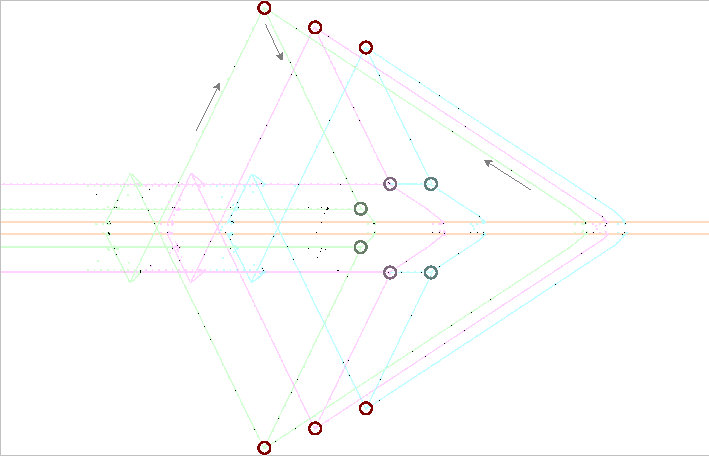
\includegraphics[width=\textwidth]{self_support_spaceships/31c_240_track_builder.pdf}}
	\caption{A configuration of rakes that uses multiple rakes and kickback reactions (circled in \bgbox{redback}{red}) to turn a $2$-block track (highlighted in \bgbox{orangeback2}{orange}) into a $6$-block track. The locations where gliders collide to synthesize the new block tracks are circled near the center.}\label{fig:31c_240_track_builder}
\end{figure}
% EXERCISE TODO: Some unhighlighted cells near center. What are they/what do they do?

However, we still do not have a method of constructing the two other block tracks, since there is no way to arrange kickback reactions so as to put gliders in front of the frontmost rakes. While this may seem like an insurmountable problem at first, one solution is to synthesize light, middle, and/or heavyweight spaceships that travel in the same direction as the Herschels, and then bounce gliders off of those rows of xWSSs.

While this approach works, instead of bouncing a glider back toward the front of the Herschels so as to synthesize the block track, we convert that glider into a middleweight spaceship via the reaction illustrated in Figure~??. The reason for this is that a middleweight spaceship can stabilize the front of the Herschel track in the exact same way as a block (in fact, one of the Herschel's sparks simply converts the MWSS into a block in the correct position), as illustrated in Figure~??.

% Two figures, side by side.

At this point, we have essentially everything that we need.

% Talk about how majority of the length of the Silverfish comes from the numerous steps needed to synthesize the HWSS pair. Then come back to this observation in Caterpillar section. Also, majority of width comes from how close we can put frontmost forward rake.

% TODO: Break this section into subsections. "Herschel crawlers and rakes", "synthesizing block trails", "synthesizing the HWSS pairs"?

\begin{figure}[!htb]
	\centering
	\embedlink{silverfish}{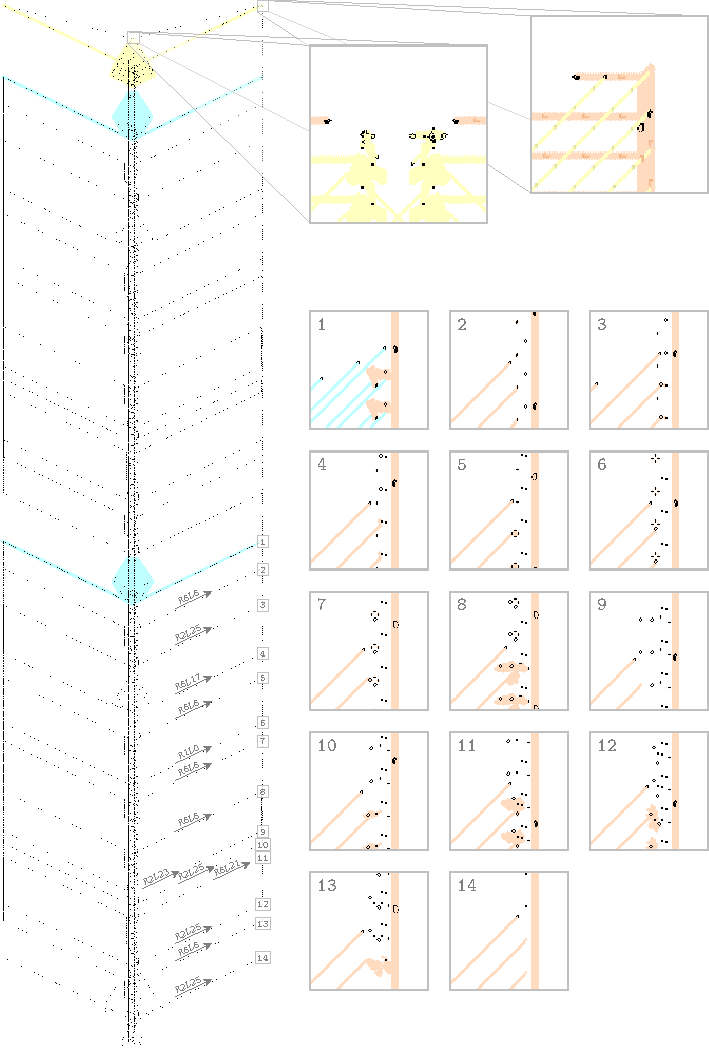
\includegraphics[width=\textwidth]{self_support_spaceships/silverfish.pdf}}
	\caption{The completed \emph{silverfish}: a $31c/240$ orthogonal spaceship, oriented so that it travels up. The track-building mechanism from Figure~\ref{fig:31c_240_track_builder} is highlighted in \bgbox{yellowback2}{yellow}. This is not done yet.}\label{fig:silverfish}
\end{figure}

% IN MAKE FORERAKES SECTION:
% R1L0F is default rake (lane 0)
% FTB in silverfish: custom 2-sync rake
% R6L6F
% R2L25F
% R6L17F
% R6L6F again
% R1L0F
% R6L6F again
% R6L6F again
% R2L23F
% R2L25F (again, the one with ponds)
% R6L21F
% R2L25F again
% R6L6F again
% R2L25F again

% R5L1F NEVER USED (maybe make an exercise with it? Like why it's not so useful? (answer: lane 1 can be reached by R2L23F in just 3 lengths instead of 5 anyway))
% R2L16 NEVER USED
% Uses 6 different forerakes total (plus the custom double forerake)


% Nivasch article: http://www.gabrielnivasch.org/fun/life/caterpillar
%%%%%%%%%%%%%%%%%%%%%%%%%%%%%%%%
\section{The Caterpillar}\label{sec:caterpillar}
%%%%%%%%%%%%%%%%%%%%%%%%%%%%%%%%

We saw another reaction that can be used to construct a self-supporting spaceship way back in Figure~\ref{fig:17c45_reaction}: a blinker can be used to move a pi-heptomino forward by $17$~cells over the course of $45$~generations (while just repositioning, not destroying, the blinker). By placing a row of blinkers with a spacing of $17$~cells as in Figure~\ref{fig:reburnable_blinker_wick}, we thus get a reburnable blinker wick that a pi-heptomino can burn through.

\begin{figure}[!htb]
	\centering
	\patternimglink{0.075}{reburnable_wick}
	\caption{A reburnable blinker wick, along which a pi-heptomino fuse (highlighted in \bgbox{greenpastel}{green}) can move at a speed of $17c/45$. The cells highlighted in \bgbox{redback}{red} make up a large spark that simply dies without affecting anything else.}\label{fig:reburnable_blinker_wick}
\end{figure}

% Redo the next 2 paragraphs in light of earlier Silverfish

A single pi-heptomino shifts the blinker wick backward by $6$~cells and rephases it,\footnote{Since the blinker wick is infinitely long, it is perhaps better to think of the pi-heptomino as shifting the wick forward by $11$~cells and not rephasing it} so if we were to place 34 pi-heptominoes on this reburnable wick then it would be moved back by $6 \times 34 = 204$ cells (which, due to the spacing of the blinkers, leaves them all exactly where they would be if no pi-heptominoes burned through them at all).\footnote{If we used just $17$ pi-heptominoes instead, the blinkers would return to their original positions, but in the opposite phases.} This gives us an infinitely-long pattern that moves at a speed of $17c/45$---our goal is to turn this into a finite configuration (i.e., a spaceship) that moves at the same speed.

To this end, we need a way of constructing the blinkers in front of the pi-heptominoes that burn through them. Fortunately, blinkers are fairly easy to construct---we can collide spaceships like gliders together so as to synthesize them. To actually \emph{create} those spaceships, we notice that the large spark that the pi-heptomino leaves behind as it burns can be collided with itself to create gliders, as demonstrated in Figure~??.

% FIGURE

% Have a section on helices here. Note that they are required when the reaction moves faster than c/4 (like here, but unlike Silverfish)


%%%%%%%%%%%%%%%%%%%%%%%%%%%%%%%%
\section{Other Self-Supporting Spaceships}\label{sec:other_self_support}
%%%%%%%%%%%%%%%%%%%%%%%%%%%%%%%%

Provide the key reactions here. Maybe one quick section for each.



%%%%%%%%%%%%%%%%%%%%%%%%%%%%%%%%
\section{Notes and Historical Remarks}\label{sec:self_support_history}
%%%%%%%%%%%%%%%%%%%%%%%%%%%%%%%%

Stuff.

% 3c/10 reaction (ref figure in chapter 1), why it hasn't worked yet. See Dave's write-up at https://www.conwaylife.com/forums/viewtopic.php?f=15&t=3427



%%%%%%%%%%%%%%%%%%%%%%%%%%%%%%%%%
\section*{Exercises \hfill \normalfont\textsf{\small solutions on \hyperlink{solutions_self_support_spaceships}{page \pageref{solutions_self_support_spaceships}}}}
\label{sec:solutions_self_support_spaceships}
\addcontentsline{toc}{section}{Exercises}
\vspace*{-0.4cm}\hrulefill\vspace*{-0.3cm}\footnotesize\begin{multicols}{2}\vspace*{-0.4cm}\raggedcolumns\interlinepenalty=10000
\setlength{\parskip}{0pt}
%%%%%%%%%%%%%%%%%%%%%%%%%%%%%%%%%


\begin{problem}\label{exer:self_support_spaceships_ex1}
	An exercise could be placed here.
\end{problem}


\mfilbreak


\begin{problem}\label{exer:self_support_spaceships_ex2}
	Another exercise could be placed here.
\end{problem}


%% EXERCISE END COMMANDS
\end{multicols}
\normalsize\vspace*{0.01cm}
%% DONE EXERCISE END COMMANDS